\providecommand{\toplevelprefix}{../..}  %
\documentclass[../../book-main_ro.tex]{subfiles}

\begin{document}

\chapter{Studiul viitor al inteligenței}
\label{ch:future}


  

\begin{quote}
``{\em Studiul urmează să fie realizat pe baza conjecturii că fiecare aspect al învățării sau orice altă caracteristică a inteligenței poate fi în principiu descris atât de precis încât o mașină poate fi făcută să îl simuleze. Se va încerca să se descopere cum să facă mașinile să folosească limbajul, să formeze abstracții și concepte, să rezolve tipuri de probleme acum rezervate oamenilor și să se îmbunătățească pe ele însele.}''

$~$\hfill -- Propunere pentru programul de IA Dartmouth, 1956
 \end{quote}
\vspace{5mm}


În general vorbind, acest manuscris este menit să introducă sistematic principii matematice și mecanisme computaționale pentru modul în care memoria sau cunoașterea pot fi dezvoltate din observații empirice. Capacitatea de a căuta parsimonie într-o lume aparent aleatorie este o caracteristică fundamentală a oricărei inteligențe, naturale sau artificiale. Credem că principiile și mecanismele prezentate în această carte sunt destul de unificatoare și universale și sunt aplicabile atât animalelor, cât și mașinilor.

Sperăm că această carte poate ajuta cititorii să clarifice pe deplin misterul din jurul practicilor moderne de rețele neuronale artificiale profunde prin dezvoltarea unei înțelegeri riguroase a funcțiilor și rolurilor lor în atingerea obiectivului de învățare a distribuțiilor de dimensiune mică din date de dimensiune mare. Cu o astfel de înțelegere, ar trebui să devenim destul de clari atât despre capacitățile, cât și despre limitările modelelor și sistemelor AI existente:
\begin{enumerate}
    \item Modelele și sistemele existente sunt departe de a fi complete în ceea ce privește un sistem de memorie care este capabil de auto-învățare și auto-îmbunătățire.
    \item Realizările existente ale acestor funcții sunt încă destul de primitive și prin forță brută și cu siguranță departe de a fi optime în ceea ce privește strategiile de optimizare și, prin urmare, arhitecturile de rețea.
    \item Modelele AI existente învață doar distribuția datelor și efectuează inferență inductivă (bayesiană), care este diferită de inteligența umană de nivel înalt.
\end{enumerate} 

Unul dintre obiectivele acestei cărți este ca oamenii să stabilească o înțelegere obiectivă și sistematică a tehnologiilor actuale de inteligență artificială și să realizeze ce probleme deschise și provocări rămân în față pentru avansarea ulterioară a inteligenței artificiale. În ultimul capitol al cărții, oferim câteva dintre punctele noastre de vedere și proiecții pentru viitor.

\section{Către inteligența autonomă: Închiderea buclei?}
Din practica inteligenței artificiale din ultimul deceniu, a devenit clar că, dacă ar exista suficiente date și resurse computaționale, s-ar putea construi un model suficient de mare și să-l pre-antrenezi pentru a învăța distribuția {\em a priori} a tuturor datelor, să zicem $p(\x)$. Teoretic, un astfel de model mare poate memoriza aproape toate cunoștințele existente despre lume care au fost codificate în limbaje și texte masive. După cum am discutat la începutul cărții, într-un fel, un astfel de model mare joacă un rol similar cu ADN-ul pe care viața îl folosește pentru a înregistra și transmite cunoștințe despre lume.

Modelul și distribuția învățate în acest fel pot fi apoi folosite pentru a regenera noi eșantioane de date bazate pe aceeași distribuție. Se poate folosi, de asemenea, modelul pentru a efectua inferență (de exemplu, estimare, predicție) cu cunoștințele memorate în diferite condiții, să zicem prin eșantionarea distribuției {\em a posteriori} $p(\x\mid \y)$ sub o nouă observație $\y$. Strict vorbind, o astfel de inferență este statistică.

Orice model pre-antrenat, oricât de mare, nu poate garanta că distribuția pe care a învățat-o până acum este complet corectă sau completă. În cazul în care eșantioanele noastre $\hat{\x}_t$ din {\em a priori} curent $p_t(\x)$ sau estimările $\hat{\x}_t(\y)$ bazate pe {\em a posteriori} $p_t(\x\mid \y)$ sunt inconsistente cu adevărul $\x$, am dori foarte mult să corectăm distribuțiile învățate:
\begin{equation}
    p_t(\x) \rightarrow p_{t+1}(\x) \quad \mbox{sau}\quad p_t(\x\mid \y) \rightarrow p_{t+1}(\x\mid \y),
\end{equation}
pe baza erorii $\boldsymbol{e}_t = \x_t - \hat{\x}_t$. Aceasta este cunoscută ca corecție a erorii bazată pe feedback de eroare, un mecanism omniprezent în natură pentru învățare continuă. Cu toate acestea, după cum știm, orice model cu capăt deschis în sine nu are mecanismul de a revizui sau îmbunătăți distribuția învățată când este incorectă sau incompletă. Îmbunătățirea modelelor AI actuale depinde încă în mare măsură de implicarea umană: experimentare, evaluare și selecție. Putem numi acest proces ``selecție artificială'' a modelelor mari, spre deosebire de selecția naturală pentru evoluția vieții.

După cum am studiat mai devreme în această carte (Capitolul \ref{ch:closed-loop} în special), sistemele cu buclă închisă ne permit să aliniem o reprezentare internă cu observațiile (percepute) ale lumii externe. Poate continua să îmbunătățească distribuția învățată intern și reprezentarea sa pentru a obține consistență sau auto-consistență. Un pas imediat înainte pentru viitor este să dezvoltăm și să construim sisteme de memorie cu buclă închisă cu adevărat, așa cum se arată în Figura \ref{fig:open-to-closed}, care sunt capabile să învețe și să îmbunătățească distribuții de date mai generale în mod autonom și continuu pe baza feedback-ului de eroare.

Prin urmare, tranziția de la modelele populare actuale cu capăt deschis antrenate de la un capăt la altul la sistemele cu buclă închisă care învață continuu:
\begin{equation}
   \mbox{\textbf{modele cu capăt deschis}} \; \Longrightarrow \; 
   \mbox{\textbf{sisteme cu buclă închisă}}
\end{equation}
este cheia pentru ca mașinile să emuleze cu adevărat modul în care creierul (animal) învață și aplică cunoștințe într-o lume deschisă. Credem că
\begin{quote}
\begin{center}
        {\em modelele cu capăt deschis sunt pentru o lume închisă, oricât de mare; \\ sistemele cu buclă închisă sunt pentru o lume deschisă, oricât de mică.}
\end{center}
\end{quote}
De fapt, ``inteligența generală'' nu ar putea fi niciodată obținută prin simpla memorare a tuturor cunoștințelor existente ale lumii. În schimb, inteligența generală poate fi obținută doar având mecanismele pentru a-și îmbunătăți memoria existentă astfel încât să poată să se adapteze la orice medii și sarcini noi.

\begin{figure}[t]
    \centering    
    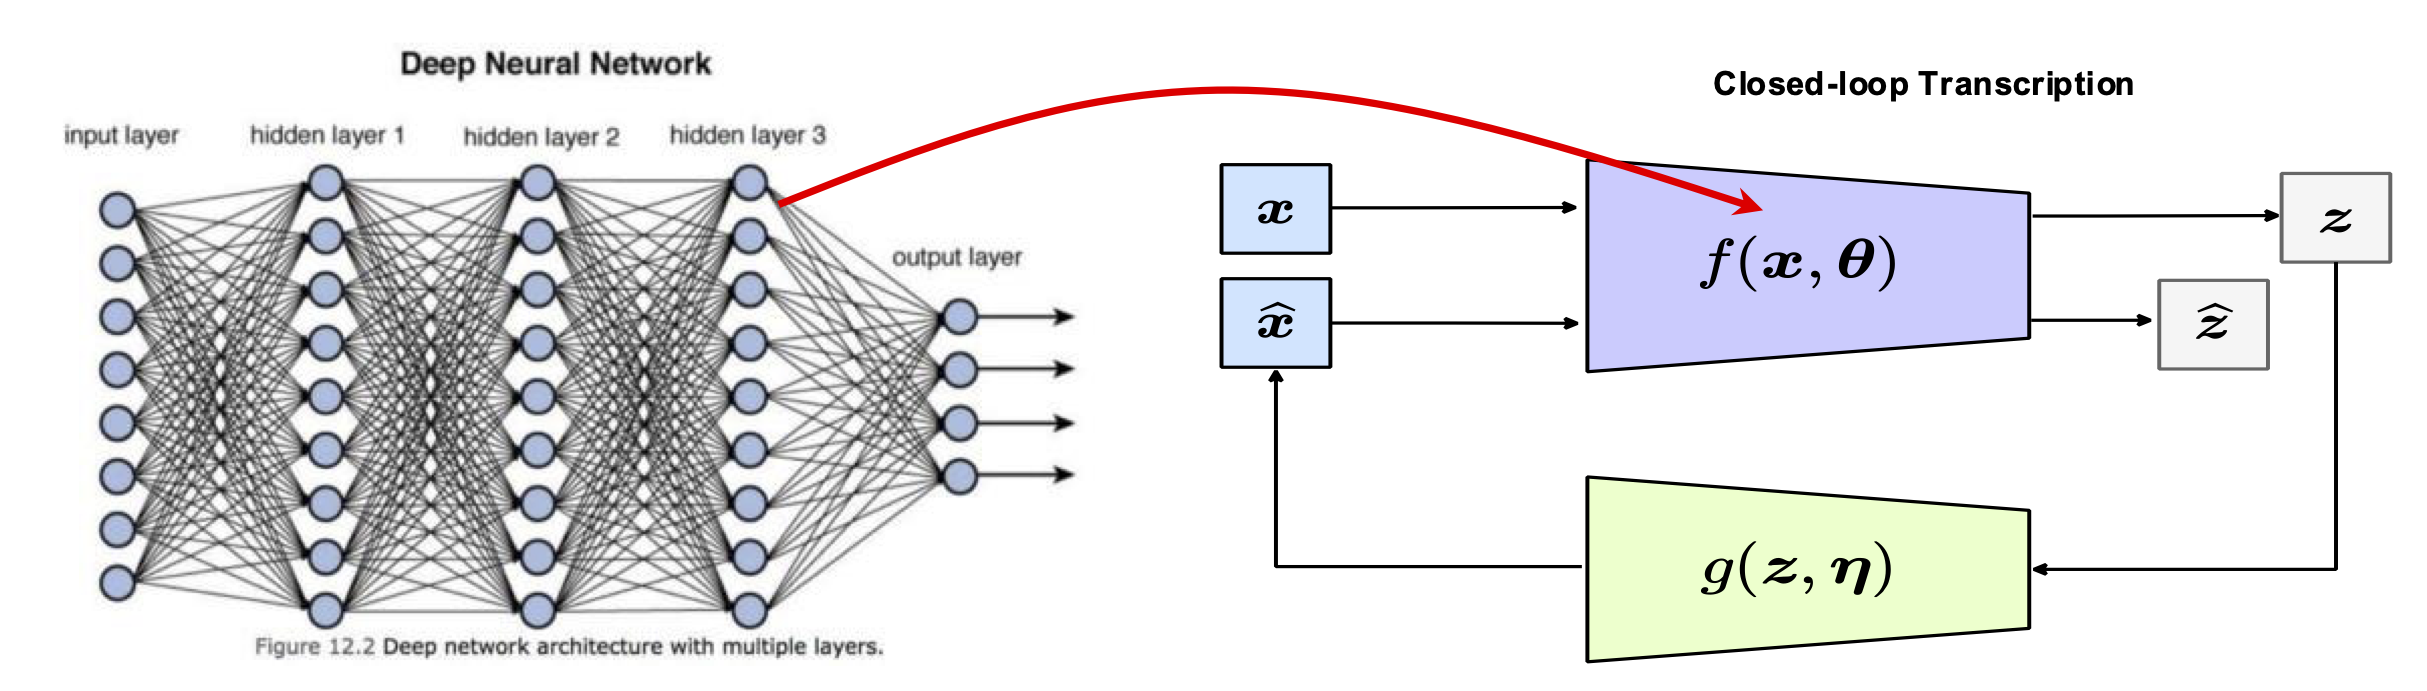
\includegraphics[width=0.9\linewidth]{\toplevelprefix/chapters/chapter8/figs/open-to-closed.png}
    \caption{De la o rețea profundă cu capăt deschis la un sistem cu buclă închisă.}
    \label{fig:open-to-closed}
\end{figure}



\section{Către inteligența naturii: Dincolo de propagarea înapoi?}
Practica inteligenței artificiale din ultimii ani i-a determinat pe mulți să creadă că trebuie să construiască un singur model mare pentru a învăța distribuția tuturor datelor și a memoriza toate cunoștințele. Chiar dacă acest lucru ar putea fi posibil din punct de vedere tehnologic, este probabil că o astfel de soluție este departe de a fi necesară și eficientă. După cum am știut din practica antrenării rețelelor profunde, singura metodă scalabilă cunoscută pentru a antrena astfel de rețele la scară este prin propagare înapoi (BP) \cite{Back-Prop}. Deși BP a oferit o modalitate de a corecta erorile prin semnale de gradient propagate înapoi prin întregul model, este totuși destul de prin forță brută și diferă semnificativ de modul în care natura învață: BP este o opțiune pe care natura nu și-o poate permite în ceea ce privește costul său ridicat sau pur și simplu nu o poate implementa din cauza limitărilor fizice.

Mai general, nu putem înțelege cu adevărat inteligența decât dacă înțelegem și cum poate fi implementată eficient. Adică, trebuie să abordăm complexitatea computațională a realizării mecanismelor asociate cu atingerea obiectivelor inteligenței. Rețineți că, din punct de vedere istoric, înțelegerea noastră a inteligenței (artificiale) a evoluat precis prin mai multe faze, de la complexitatea Kolmogorov incalculabilă la entropia lui Shannon, de la calculabilitatea lui Turing la înțelegerea ulterioară a tractabilității,\footnote{Spunem că o problemă este tractabilă dacă permite un algoritm a cărui complexitate este polinomială în dimensiunea problemei.} și la accentul puternic pe scalabilitatea algoritmului în practica modernă a inteligenței artificiale. Această evoluție poate fi rezumată ca următoarea diagramă:
\begin{equation}
   \mbox{\textbf{incalculabil}} \;
   \Longrightarrow \; \mbox{\textbf{calculabil}} \;
   \Longrightarrow \; \mbox{\textbf{tractabil}} \; \Longrightarrow \; 
   \mbox{\textbf{scalabil}}.
\end{equation}
Într-o mare măsură, succesul și popularitatea învățării profunde și a propagării înapoi se datorează precis faptului că au oferit o implementare scalabilă cu platforme de calcul moderne (cum ar fi GPU-urile) pentru procesarea și comprimarea datelor masive. Cu toate acestea, o astfel de implementare este încă mult prea scumpă în comparație cu modul în care natura realizează inteligența.

Rămâne un spațiu imens pentru îmbunătățirea eficienței inteligenței artificiale, astfel încât să poată emula nivelul de eficiență al inteligenței naturale, care ar trebui să fie cu ordine de mărime mai eficient decât implementările actuale prin forță brută. În acest scop, trebuie să descoperim noi arhitecturi de învățare și mecanisme de optimizare care să permită învățarea distribuțiilor de date în condiții fizice naturale și constrângeri de resurse, similare cu cele pentru ființele inteligente din natură, să zicem, fără a accesa toate datele simultan sau a actualiza toți parametrii modelului simultan (prin BP).

Cadrul și abordarea principială prezentate în această carte ne pot ghida să descoperim astfel de arhitecturi și mecanisme noi. Aceste arhitecturi și mecanisme noi ar trebui să permită învățarea continuă online și pot fi actualizate prin optimizare înainte sau înapoi extrem de localizată și rară. Până acum, pentru învățarea unei distribuții, singurul caz pentru care știm că există o astfel de soluție este cel mai simplu caz al PCA, cu metoda PCA online introdusă în Capitolul \ref{ch:autoencoding}.

\begin{figure}[t]
\centering
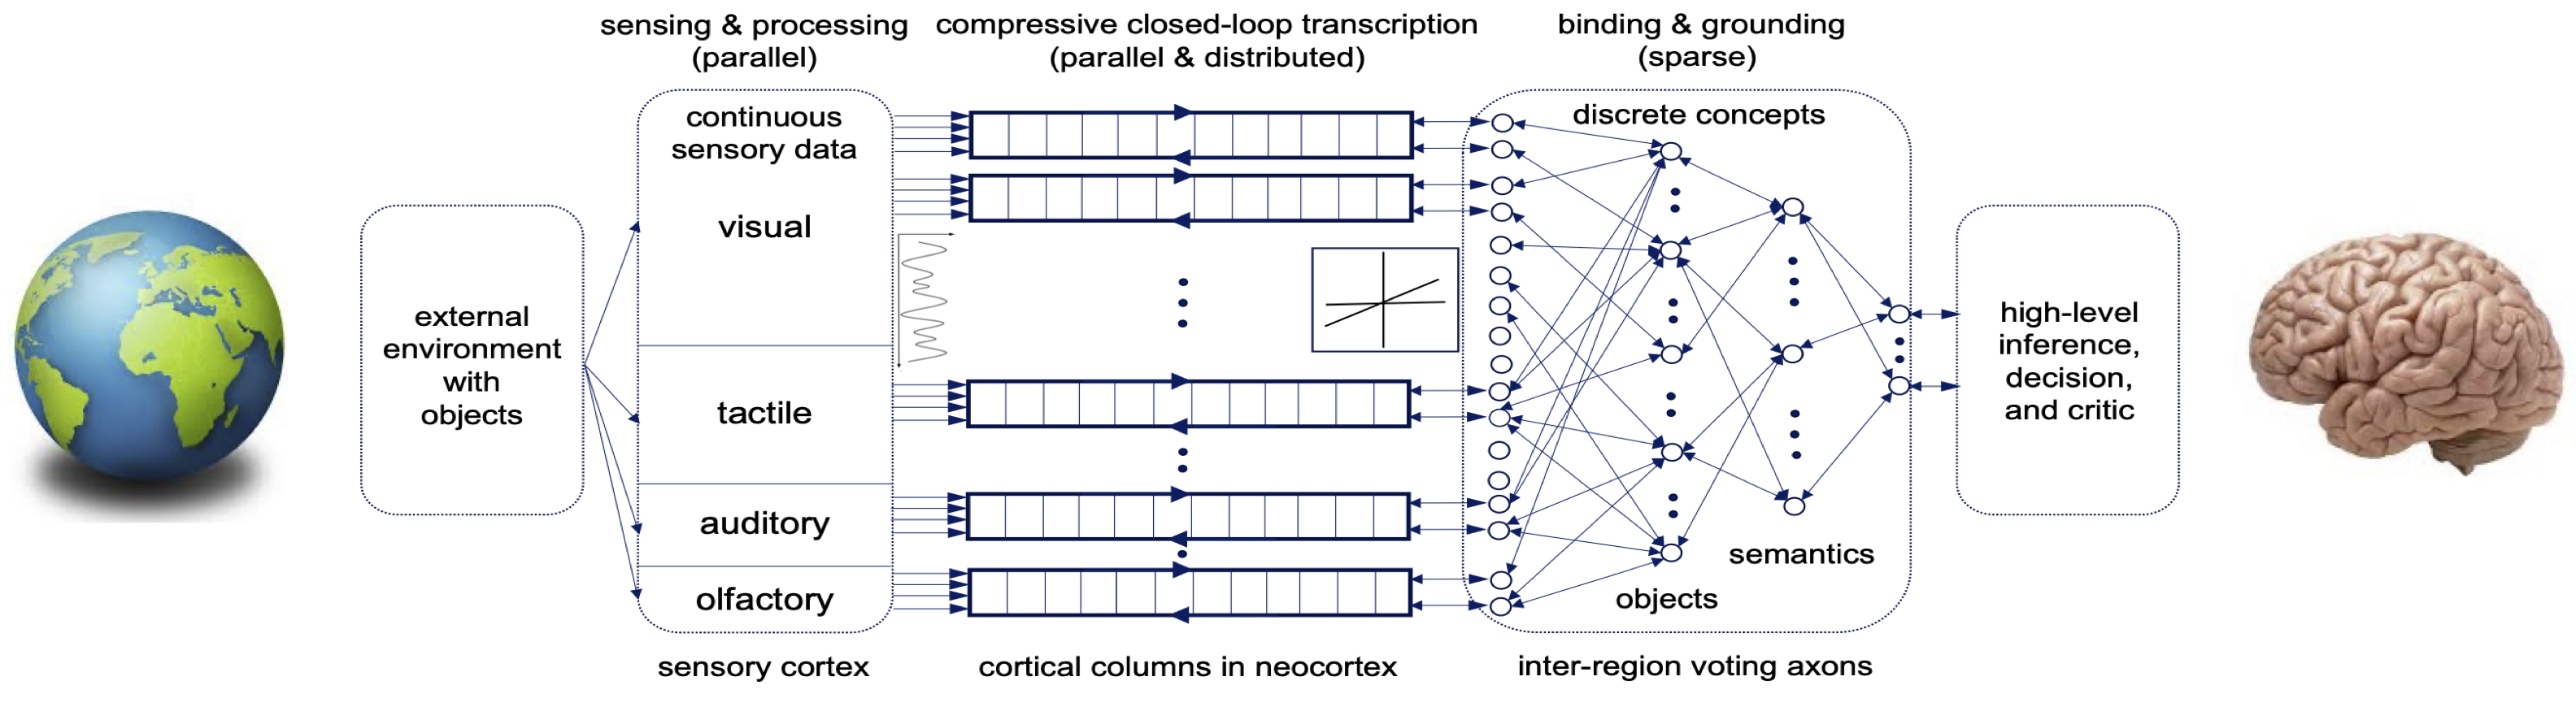
\includegraphics[width=0.99\linewidth]{\toplevelprefix/chapters/chapter8/figs/loops.png}
    \caption{Arhitectura conjecturată a cortexului cerebral: Cortexul este un sistem de auto-codare masiv paralel și distribuit care constă dintr-o ierarhie de autocodoare cu buclă închisă care extrag informații din mai multe simțuri și maximizează câștigul de informații al reprezentărilor rezultate la mai multe niveluri de ierarhie și granularitate.}
    \label{fig:loops}
\end{figure}
După cum am învățat din neuroștiință, cortexul creierului nostru constă din zeci de mii de coloane corticale. Toate coloanele corticale au structuri și funcții fizice similare. Ele sunt extrem de paralele și distribuite, deși interconectate rar. Prin urmare, credem că pentru a dezvolta un sistem de memorie mai scalabil și structurat, trebuie să luăm în considerare arhitecturi care emulează pe cele ale cortexului. Figura \ref{fig:loops} arată o astfel de arhitectură ipotezată, un sistem masiv distribuit și ierarhic care constă din multe module de auto-codare cu buclă închisă în mare parte paralele. Aceste module învață să codifice diferite modalități senzoriale sau multe proiecții ale datelor din fiecare modalitate senzorială. Discuția noastră din Secțiunea \ref{sec:measurement-self-consistency} din Capitolul \ref{ch:conditional-inference} sugerează că o astfel de detecție și învățare paralelă a unei distribuții de dimensiune mică este teoretic posibilă. Autocodoarele de nivel superior (cu pierderi) pot fi apoi învățate pe baza ieșirilor celor de nivel inferior pentru a dezvolta ``abstracții'' mai rare și de nivel superior ale reprezentărilor învățate de nivelurile inferioare.


Arhitectura de sistem distribuită, ierarhică și cu buclă închisă ilustrată în Figura \ref{fig:loops} împărtășește multe caracteristici ale cortexului cerebral. O astfel de arhitectură de sistem poate deschide mult mai multe posibilități decât arhitectura actuală cu un singur model mare. Face posibilă explorarea unor mecanisme de învățare și optimizare mult mai eficiente și are ca rezultat o organizare modulară mai structurată a distribuției datelor învățate și a cunoștințelor. Aceasta ne-ar permite să aducem implementarea inteligenței artificiale la următorul nivel de evoluție:
\begin{equation}
   \mbox{\textbf{incalculabil}} \;
   \Longrightarrow \; \mbox{\textbf{calculabil}} \;
   \Longrightarrow \; \mbox{\textbf{tractabil}} \; \Longrightarrow \; 
   \mbox{\textbf{scalabil}} \; \Longrightarrow \; 
   \mbox{\textbf{natural}}.
\end{equation}

\section{Către inteligența artificială umană: Dincolo de testul Turing?}
După cum am discutat la începutul acestei cărți, Capitolul \ref{ch:intro}, inteligența în natură a evoluat prin mai multe faze și s-a manifestat în patru forme diferite:
\begin{equation}
\mbox{\textbf{filogenetică}} \;
   \Longrightarrow \; \mbox{\textbf{ontogenetică}} \; \Longrightarrow \; 
   \mbox{\textbf{societală}}
   \; \Longrightarrow \; 
   \mbox{\textbf{inteligență artificială}}.
\end{equation}
Toate formele de inteligență împărtășesc obiectivul comun de a învăța cunoștințe utile ca anumite distribuții de dimensiune mică ale datelor de dimensiune mare percepute despre lume. Cu toate acestea, ele pot diferi semnificativ în schemele specifice de codare adoptate, informațiile codificate, mecanismele computaționale pentru învățare și îmbunătățire și implementările fizice ale acestor mecanisme. Folosind conceptele și terminologiile dezvoltate în această carte, din perspectiva învățării și reprezentării informațiilor sau cunoștințelor din distribuția datelor percepute, cele patru etape de mai sus ale inteligenței dezvoltate în natură diferă în următoarele trei aspecte:
\begin{enumerate}
    \item Cartea de coduri pe care o folosește pentru a învăța și codifica informațiile sau cunoștințele intenționate.
    \item Informațiile sau cunoștințele care sunt codificate și reprezentate folosind cartea de coduri.
    \item Mecanismele de optimizare folosite pentru a îmbunătăți informațiile sau cunoștințele codificate.
\end{enumerate}
Mai specific, următorul tabel rezumă caracteristicile lor principale în cele trei aspecte de mai sus:
\begin{center}
\begin{tabular}{| c | c | c | c | c |}
\hline & \textbf{Filogenetică} & \textbf{Ontogenetică} & \textbf{Societală} & \textbf{Artificială}\\
\hline
\textbf{Carte de coduri}  & Aminoacizi & Neuroni & Alfabet și cuvinte & Matematică/Logică \\ [0.5ex]
  \hline 
\textbf{Informație} & Gene/ADN & Memorie & Limbaje/Texte & Fapte științifice\\ [0.5ex]
  \hline
\textbf{Optimizare} & Învățare prin întărire & Feedback de eroare & Încercare și eroare & Testarea ipotezelor \\  [0.5ex]
\hline
\end{tabular}
\end{center}





După cum știm acum, oamenii au realizat două salturi cuantice în inteligență în istorie.
Primul este dezvoltarea limbajelor vorbite și scrise cu aproximativ cinci până la zece mii de ani în urmă. Aceasta a permis oamenilor să împărtășească și să transmită cunoștințe învățate pentru generații, similar cu rolul ADN-ului în natură. Al doilea este dezvoltarea matematicii și logicii cu aproximativ trei mii de ani în urmă, care au devenit un limbaj precis pentru știința modernă. Acest nou limbaj ne-a eliberat de rezumarea cunoștințelor din observații în forme empirice și ne-a permis să formalizăm cunoștințele ca teorii verificabile sau falsificabile prin deducție matematică sau verificare experimentală. Prin formularea ipotezelor, deducția logică și testarea experimentală, suntem capabili să descoperim proactiv noi cunoștințe care erau imposibile anterior prin învățarea pasivă din distribuția datelor.\footnote{cum ar fi relațiile cauzale}

După cum am discutat în Introducere (Capitolul \ref{ch:intro}), programul de ``inteligență artificială'' (IA) din 1956 a urmărit precis să studieze funcții de nivel înalt, cum ar fi abstracțiile matematice, inferența logică și rezolvarea problemelor care se crede că diferențiază oamenii de animale:
\begin{equation}
   \mbox{inteligență \textbf{de nivel scăzut} (animală)} \; \Longrightarrow \; 
   \mbox{inteligență \textbf{de nivel înalt} (umană).}
\end{equation}
După cum am clarificat în mod repetat în această carte, multe dintre progresele tehnologice în inteligența artificială din ultimele decenii, deși realizate sub numele de ``IA'', sunt de fapt mai strâns legate de inteligența de nivel scăzut împărtășită atât de animale, cât și de oameni, care este în principal inductivă. Până acum, nu au existat dovezi care să sugereze că aceste mecanisme singure ar fi suficiente pentru a obține inteligența umană de nivel înalt pe care programul original de IA urmărește cu adevărat să o înțeleagă și să o emuleze.

De fapt, știm puțin despre cum să verificăm riguros dacă un sistem este cu adevărat capabil de o anumită inteligență de nivel înalt, în ciuda faptului că testul Turing a fost propus încă din 1950 \cite{Turing-1950}.\footnote{În propunerea lui Turing, evaluatorul este un om. Cu toate acestea, pregătirea științifică și cunoștințele majorității evaluatorilor umani pot fi limitate și concluziile lor pot fi subiective.} Pentru mult timp, un astfel de test nu a fost considerat necesar, deoarece capacitățile mașinilor erau cu mult sub cele ale unui om (sau chiar animal). Cu toate acestea, având în vedere progresele tehnologice recente, multe modele și sisteme au pretins că ating și chiar depășesc inteligența umană. Prin urmare, este timpul să dăm o definiție științifică și executabilă a testului Turing. Adică, cum evaluăm sistematic și obiectiv nivelul de inteligență pentru un model sau sistem dat? De exemplu, cum putem verifica riguros dacă un sistem inteligent a înțeles cu adevărat un anumit concept abstract, cum ar fi noțiunea de numere naturale sau reale, sau a memorat doar un număr mare de instanțe? Rețineți că modelele de limbaj de ultimă generație încă se luptă cu întrebări matematice simple precum: ``3.11 este mai mare sau mai mic decât 3.9?''\footnote{Rețineți că unele modele și-au corectat răspunsurile la întrebări de acest gen prin inginerie post. Sau unele modele au încorporat mecanisme de raționament suplimentare bazate pe verificarea răspunsurilor imediate produse și corectarea lor în timpul raționamentului. Cu toate acestea, lăsăm cititorului ca exercițiu să testeze riguros dacă vreunul dintre modelele de limbaj de ultimă generație înțelege cu adevărat noțiunea de numere (naturale, raționale, reale și complexe) și aritmetica asociată.}
Cum verificăm dacă un sistem înțelege cu adevărat regulile logicii și știe cum să le aplice riguros sau a memorat pur și simplu un număr mare de instanțe de practică a logicii? Mai mult, este un astfel de sistem chiar capabil să-și corecteze propriile cunoștințe sau să dezvolte noi cunoștințe, cum ar fi legi fizice, concepte matematice sau relații cauzale? În rezumat, este timpul să dezvoltăm metode riguroase de evaluare care pot spune căruia dintre următoarele aparține capacitatea aparent inteligentă a unui sistem/model:
\begin{enumerate}
    \item pur și simplu a memorat distribuția unor date purtătoare de cunoștințe și o regenerează;
    \item poate dezvolta autonom și continuu noi cunoștințe din observații noi;
    \item a înțeles cu adevărat anumite cunoștințe abstracte și știe cum să le aplice corect;
    \item poate genera noi ipoteze științifice sau conjecturi matematice și să le verifice.
\end{enumerate}

\begin{figure}[t]
    \centering
    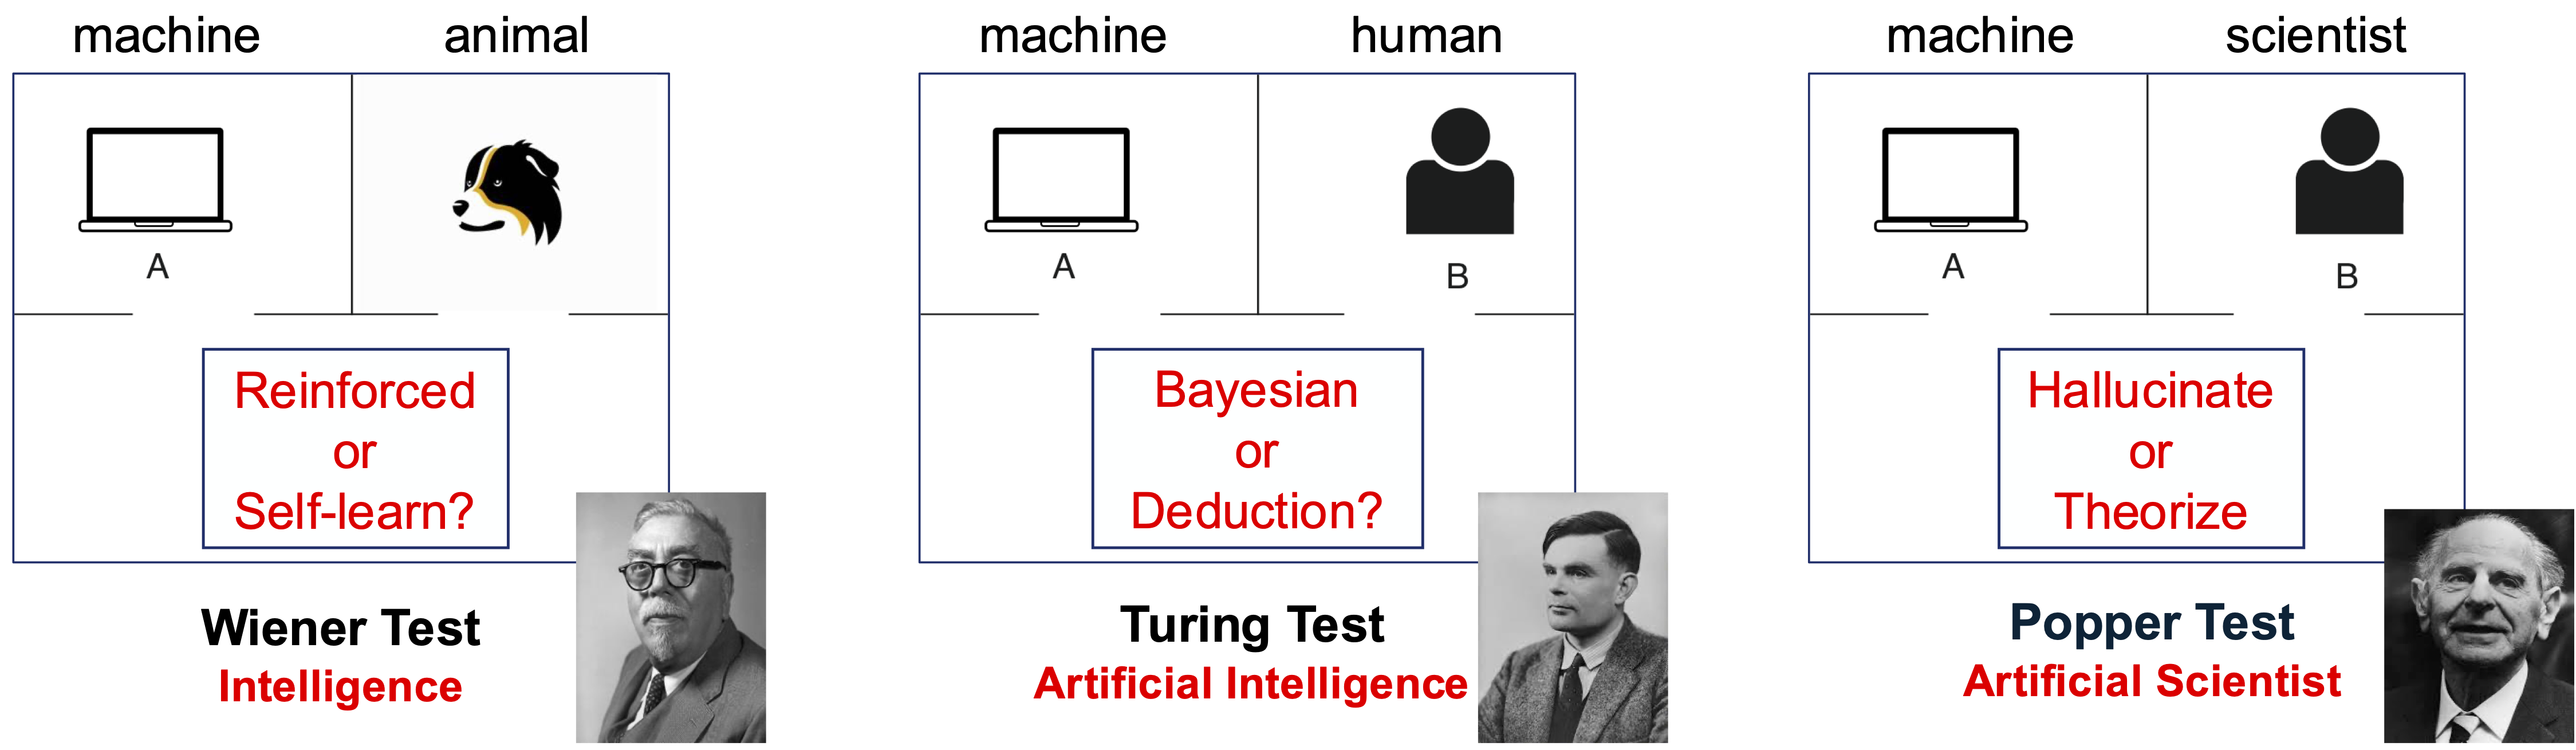
\includegraphics[width=0.95\linewidth]{\toplevelprefix/chapters/chapter8/figs/tests.png}
    \caption{Trei teste pentru diferite niveluri sau tipuri de capacități de inteligență: testul Wiener pentru inteligența de bază, testul Turing pentru inteligența artificială la nivel uman și testul Popper pentru inteligența la nivel de om de știință.}
    \label{fig:three-tests}
\end{figure}

Figura \ref{fig:three-tests} ilustrează că probabil ar trebui să existe cel puțin trei tipuri diferite de teste pentru a evalua și diferenția diferite tipuri de capacități de inteligență:
\begin{enumerate}
    \item {\em Testul Norbert Wiener:} Pentru a evalua dacă un sistem este capabil să îmbunătățească și să dezvolte noi cunoștințe proprii sau pur și simplu primește informații prin învățare întărită sau supervizată;
    \item {\em Testul Alan Turing:} Pentru a evalua dacă un sistem poate înțelege cunoștințe abstracte sau pur și simplu învață statisticile sale și le folosește pentru inferență bayesiană.
    \item {\em Testul Karl Popper:} Pentru a evalua dacă un sistem este capabil să exploreze noi cunoștințe prin formarea și verificarea de noi teorii bazate pe auto-consistență.
\end{enumerate}
Credem că, pentru astfel de metode de evaluare, evaluatorul nu ar trebui să fie un om, ci mai degrabă un protocol și un proces științific solid.



După cum am văzut pe parcursul acestei cărți întregi, {\em compresia} a jucat un rol cel mai fundamental în învățare. Este principiul guvernator și un mecanism unificat pentru identificarea unei distribuții de date (empirice) și organizarea informațiilor codificate în ea. Într-o mare măsură, explică cea mai mare parte a practicii ``inteligenței artificiale'' din ultimul deceniu sau cam așa ceva. Aici cuvântul ``artificial'' înseamnă în mare parte ``făcut de om''. O întrebare remarcabilă pentru studiul viitor este dacă {\em compresia singură} este suficientă pentru a obține toate capacitățile de nivel superior ale inteligenței enumerate mai sus.
\begin{quote}
\begin{center}
        {\em Este compresia tot ce există?}
\end{center}
\end{quote}
Sunt abstracția, inferența cauzală, raționamentul logic și generarea de ipoteze și deducția ulterioară anumite forme extinse sau extreme de compresie? Există o diferență fundamentală între identificarea distribuțiilor de date empirice prin compresie și formarea de concepte și teorii abstracte de nivel înalt? Filozoful Sir Karl Popper a sugerat odată:
\begin{quote}
    \begin{center}
    {\em ``Știința poate fi descrisă ca arta simplificării sistematice excesive.''}
    \end{center}
\end{quote}
Într-o mare măsură, știința și cartea sa de coduri asociată, matematica, pot fi văzute ca cea mai avansată formă de inteligență, prin urmare, partea cu adevărat ``artificială'' a inteligenței noastre. Aici cuvântul ``artificial'' înseamnă ceea ce este unic pentru oamenii educați și iluminați, aproape ca o formă de artă înaltă. Credem că descoperirea și înțelegerea principiilor matematice de bază și a mecanismelor computaționale ale unei astfel de inteligențe de nivel superior vor fi frontiera finală pentru Știință, Matematică și Calcul în totalitate!

\end{document}